% !TEX root = ../main.tex
\chapter{Kiến trúc Tổng thể và Luồng Hoạt động CRAG}

\section{Kiến trúc 3 Layer Tách Biệt}

Kiến trúc phiên bản V3 được chuẩn hóa thành 3 tầng chức năng độc lập, phân định ranh giới rõ ràng giữa Giao diện, Xử lý tác tử và Cơ sở dữ liệu.

\begin{figure}[htbp]
    \centering
    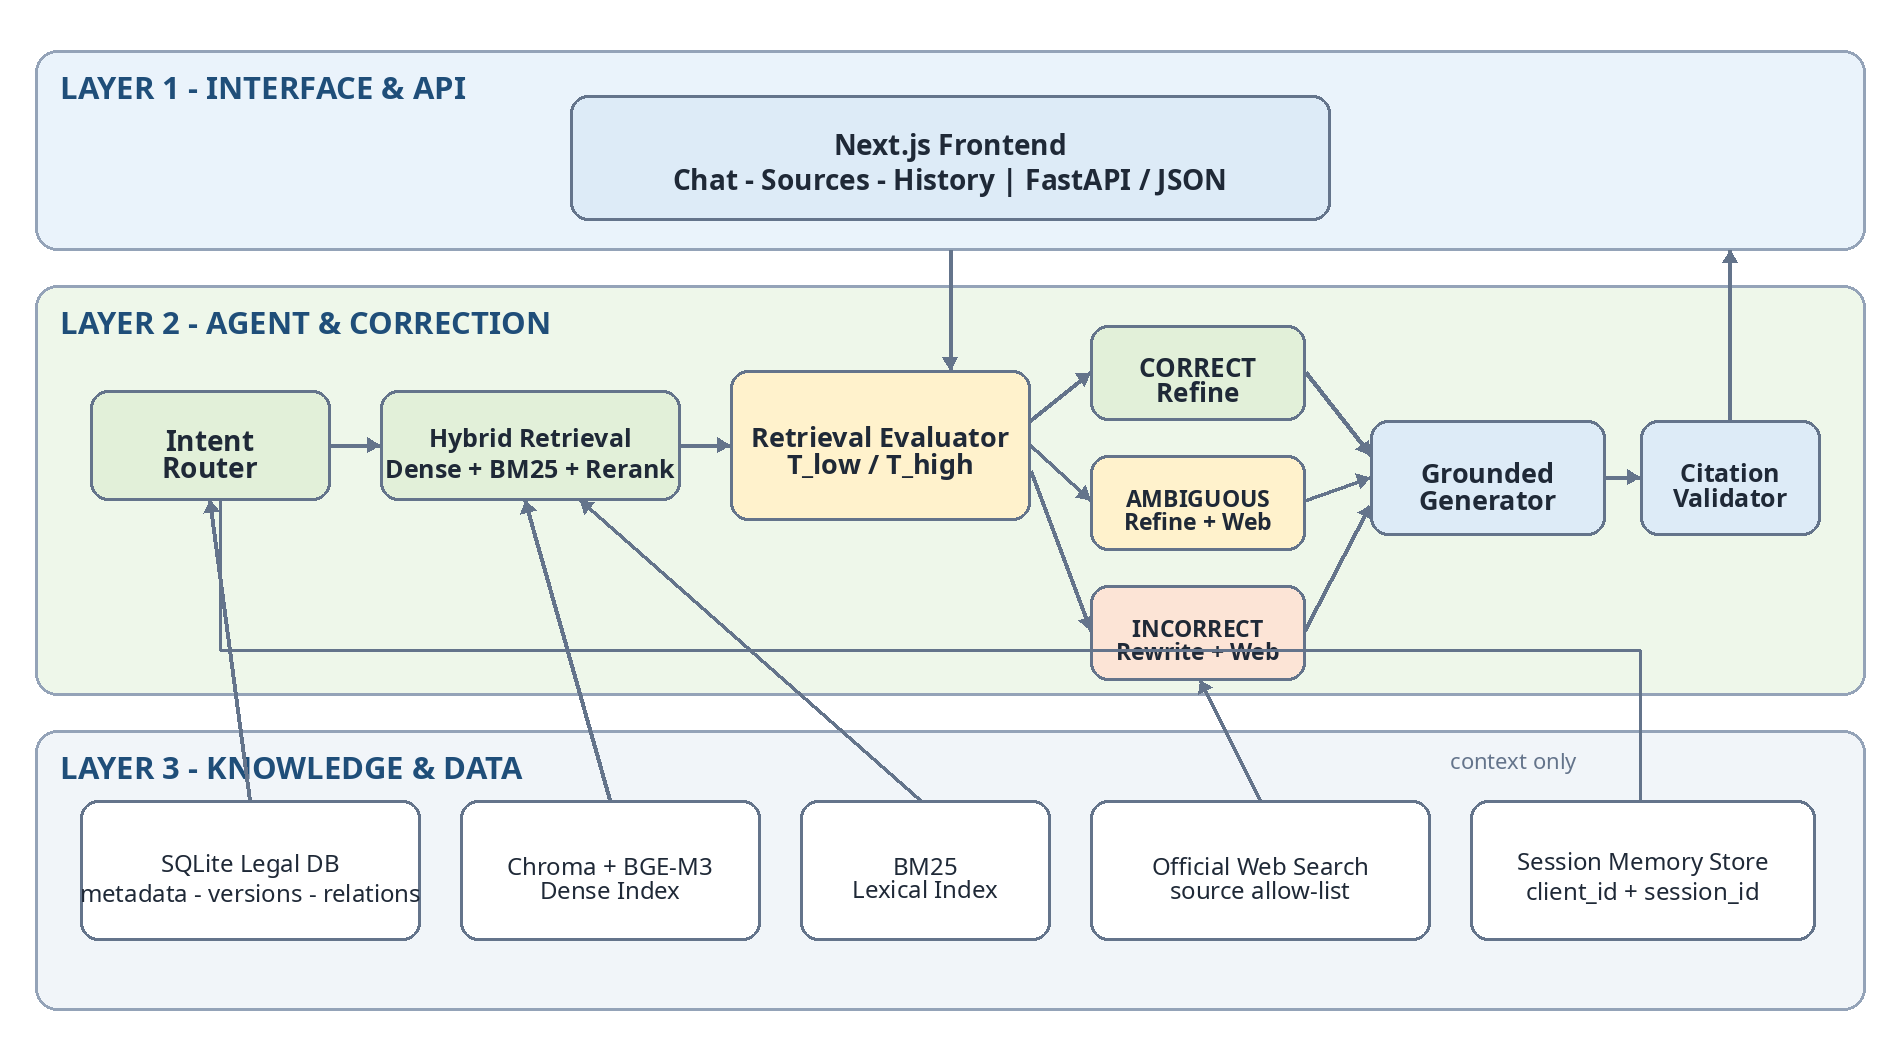
\includegraphics[width=0.92\textwidth]{images/figure_1.png}
    \caption{Kiến trúc 3 Layer của Legal CRAG Agent V3.}
    \label{fig:arch_3layer}
\end{figure}

\begin{table}[htbp]
\centering
\caption{Phân định chức năng và vai trò của từng Layer trong hệ thống}
\label{tab:layer_roles}
\renewcommand{\arraystretch}{1.3}
\rowcolors{2}{tablerowalt}{white}
\begin{tabularx}{\textwidth}{L{4.2cm} Y}
\toprule
\rowcolor{tableheader}\color{white}\textbf{Layer / Khối chức năng} & \color{white}\textbf{Vai trò và Trách nhiệm chính} \\
\midrule
\textbf{Layer 1 -- Interface \& API} & Next.js + TypeScript phụ trách giao diện người dùng chuyên nghiệp; FastAPI cung cấp hạ tầng RESTful/JSON API kết nối trực tiếp với Agent, hỗ trợ hiển thị câu trả lời, bảng trích dẫn citation, danh mục source và quản lý phiên. \\
\textbf{Layer 2 -- Agent \& Correction} & LangGraph điều phối toàn bộ workflow: Router phân loại câu hỏi, Retrieval Evaluator chấm điểm, 3 nhánh xử lý CRAG cốt lõi, Generator và Citation Validator đảm bảo độ chính xác. \\
\textbf{Layer 3 -- Knowledge \& Data} & SQLite quản lý metadata pháp lý và lịch sử phiên, Chroma DB lưu trữ dense vector index, BM25 lưu lexical index, Reranker tính toán relevance, và công cụ Controlled Web Search với danh sách nguồn cho phép. \\
\bottomrule
\end{tabularx}
\end{table}

\section{Luồng Hoạt động CRAG Cốt lõi (3 Nhánh)}

Trọng tâm của kỹ thuật Corrective RAG là không bao giờ tin tưởng tuyệt đối vào kết quả truy hồi ban đầu. Thay vào đó, một bộ đánh giá (\textit{Retrieval Evaluator}) sẽ phân loại tập tài liệu truy hồi thành một trong ba trạng thái:

\begin{figure}[htbp]
    \centering
    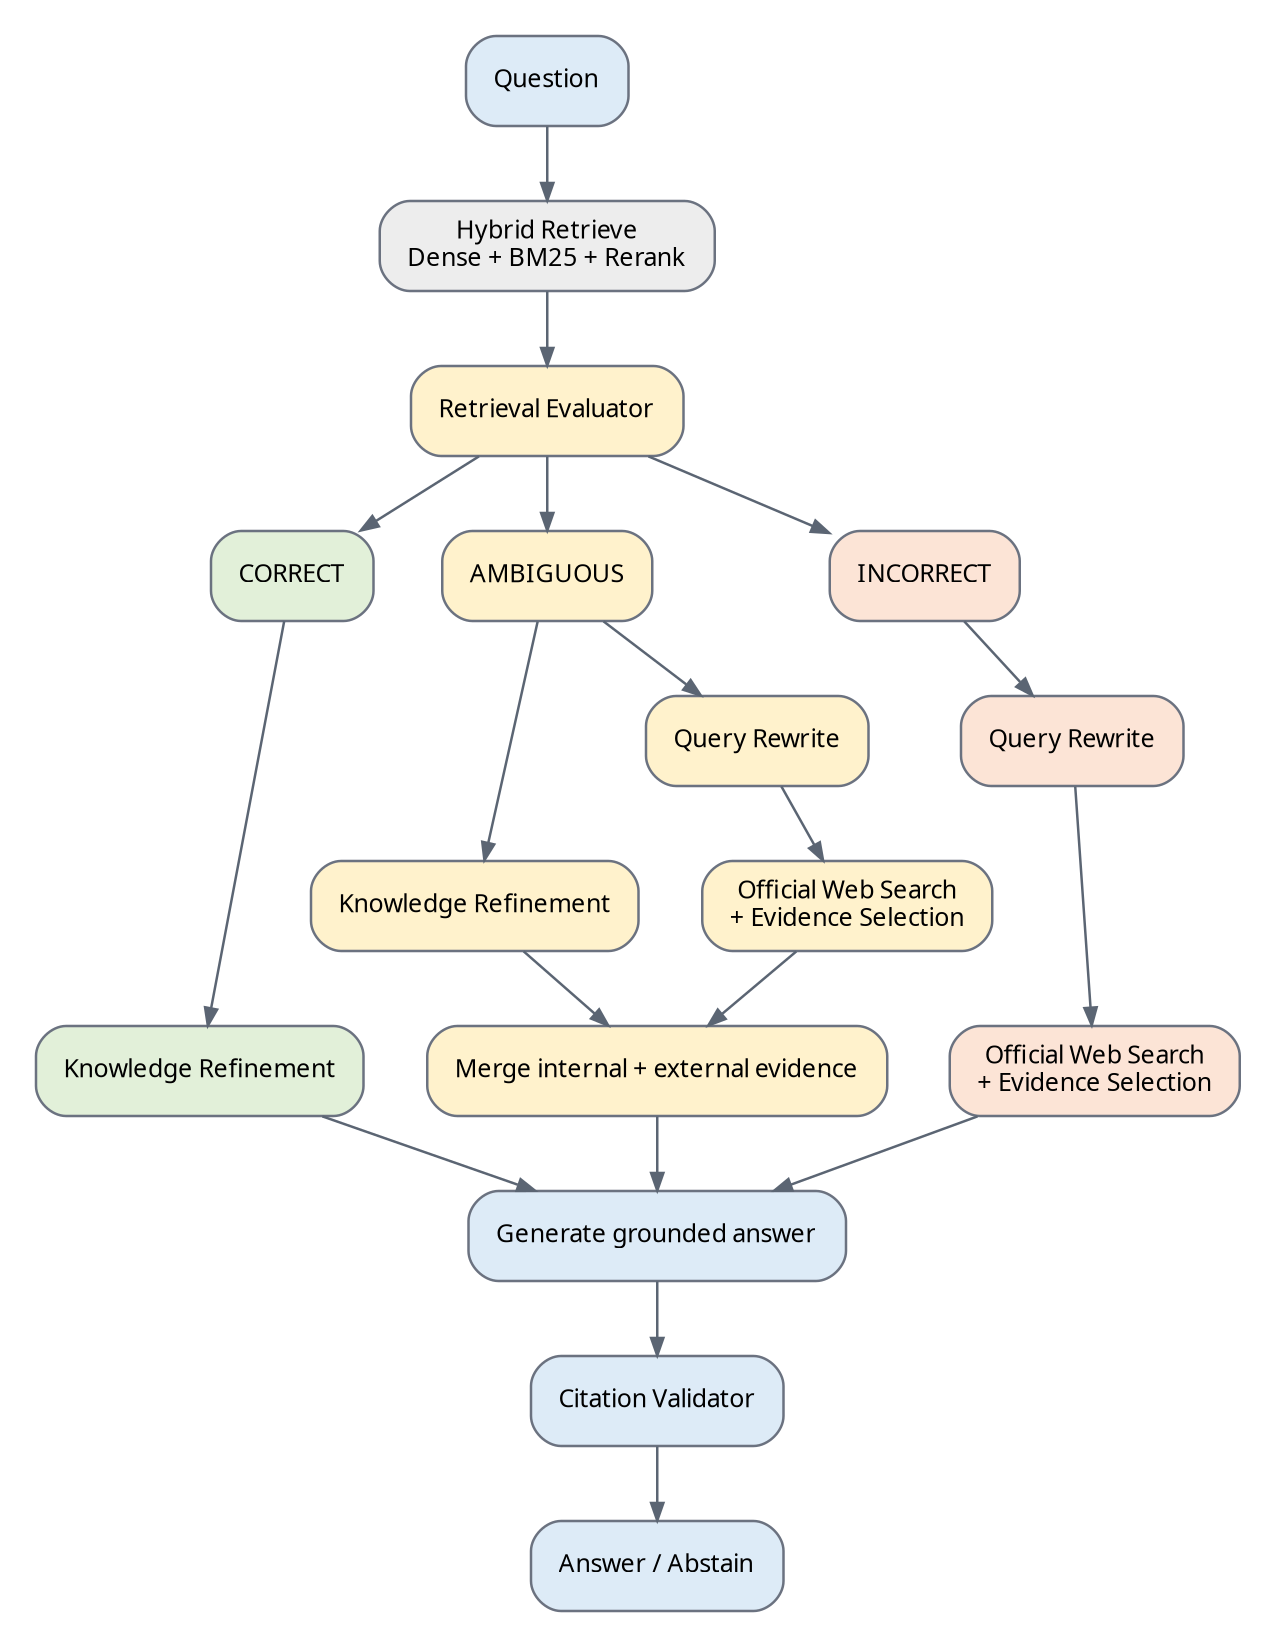
\includegraphics[width=0.75\textwidth]{images/figure_2.png}
    \caption{Luồng xử lý 3 nhánh Correct / Ambiguous / Incorrect theo nguyên lý CRAG.}
    \label{fig:crag_workflow}
\end{figure}

\begin{itemize}
    \item \textbf{Nhánh CORRECT (Tài liệu đạt chuẩn):} Điểm liên quan cao vượt ngưỡng $T_{high}$. Hệ thống kích hoạt \textit{Knowledge Refinement} để bóc tách các điều khoản (legal strips) trực tiếp trả lời câu hỏi, loại bỏ nhiễu và chuyển sang bộ sinh câu trả lời.
    \item \textbf{Nhánh INCORRECT (Tài liệu không phù hợp/thiếu hụt):} Điểm liên quan tối đa nằm dưới ngưỡng $T_{low}$. Hệ thống xác định corpus nội bộ không có căn cứ, loại bỏ toàn bộ tài liệu rác, thực hiện \textit{Query Rewrite} thành truy vấn tìm kiếm chuẩn mực và gọi công cụ \textit{Controlled Web Search} qua các cổng thông tin pháp luật chính thống.
    \item \textbf{Nhánh AMBIGUOUS (Tài liệu không rõ ràng/chưa đủ):} Điểm liên quan nằm giữa khoảng $[T_{low}, T_{high})$. Hệ thống vừa tinh chế tài liệu nội bộ, vừa viết lại truy vấn để tìm kiếm bổ sung trên web, sau đó tiến hành \textit{Evidence Merging} hợp nhất và khử trùng lặp trước khi sinh lời giải.
\end{itemize}

\begin{calloutbox}{Điểm cải tiến then chốt so với các thiết kế cũ}
Các phiên bản trước thường đưa nhánh \textit{Ambiguous} quay lại vòng lặp truy hồi (\textit{looping}) với biến \texttt{MAX\_ITER}. Thiết kế V3 loại bỏ việc lặp lại máy móc: nhánh Ambiguous bắt buộc phải kết hợp tinh lọc tri thức nội bộ và mở rộng nguồn web có kiểm soát, giải quyết dứt điểm vấn đề thiếu bằng chứng mà không gây lặp vô hạn.
\end{calloutbox}

\section{Stack Công nghệ Đề xuất}

\begin{table}[htbp]
\centering
\caption{Chi tiết Stack công nghệ triển khai hệ thống Legal CRAG V3}
\label{tab:tech_stack}
\renewcommand{\arraystretch}{1.25}
\rowcolors{2}{tablerowalt}{white}
\begin{tabularx}{\textwidth}{L{3.5cm} L{4.5cm} Y}
\toprule
\rowcolor{tableheader}\color{white}\textbf{Thành phần} & \color{white}\textbf{Công nghệ lựa chọn} & \color{white}\textbf{Lý do và Ghi chú kỹ thuật} \\
\midrule
Ngôn ngữ nền tảng & Python 3.11+ & Đảm bảo tính tương thích cao với LangGraph, PyTorch và transformers. \\
LLM Engine & Đa Provider (Groq, OpenAI, OpenRouter, Ollama) & Kiến trúc Factory linh hoạt: Groq (siêu tốc), OpenAI GPT-4o, OpenRouter và Ollama (local on-premise); cấu hình qua \texttt{LLM\_PROVIDER}; cố định \texttt{temperature=0}. \\
Embedding Model & BAAI/BGE-M3 & Embedding đa ngữ mạnh mẽ, xử lý tốt văn bản pháp luật tiếng Việt. \\
Dense Vector DB & ChromaDB & Nhẹ, nhúng trực tiếp, tối ưu cho quy mô 50--100 văn bản pháp lý. \\
Lexical Retrieval & rank-bm25 (BM25Okapi) & Bù đắp exact-match chính xác cho số hiệu văn bản, số Điều/Khoản. \\
Reranker & BAAI/bge-reranker-v2-m3 & Cross-encoder tính relevance score chuẩn xác cho Retrieval Evaluator. \\
Agent Orchestrator & LangGraph & Điều phối workflow dạng đồ thị có trạng thái (\textit{StateGraph}) và rẽ nhánh điều kiện. \\
Cơ sở dữ liệu & SQLite & Quản lý quan hệ văn bản, phiên bản điều luật, session logs và memory. \\
Web Search & Custom Engine + Allow-list & Chỉ thu thập từ các tên miền công quyền: \texttt{vbpl.vn}, \texttt{chinhphu.vn}... \\
Đánh giá chất lượng & RAGAS + Custom Metrics & Đo lường Faithfulness, Citation Accuracy và Legal Temporal Correctness. \\
Theo dõi & LangFuse & Ghi nhận toàn bộ vết thực thi, latency và chi phí token của từng node. \\
Frontend & Next.js + TypeScript & Giao diện tra cứu hiện đại, hiển thị bảng bằng chứng và lịch sử hội thoại. \\
API Gateway & FastAPI + Uvicorn & Cung cấp API chuẩn hóa REST/JSON kết nối UI và LangGraph Agent. \\
\bottomrule
\end{tabularx}
\end{table}
